\documentclass[fleqn,10pt]{wlscirep}
\usepackage[utf8]{inputenc}
\usepackage[T1]{fontenc}
\usepackage{enumerate}
\usepackage{float} % keeps tables in the exact position they occupy in the code
\usepackage{natbib}
\usepackage{adjustbox}
\usepackage{graphicx}
\usepackage{subcaption}
\usepackage{pifont}
\usepackage{gb4e} % leave last

\title{Parametric settings of functional projections in diachrony: French wh-interrogatives and clefts}

\author[1,*]{Caterina Bonan}
\author[2]{Giuseppe Samo}
% \author[1,2,+]{Christine Author}
% \author[2,+]{Derek Author}
\affil[1]{University of Cambridge, United Kingdom.}
\affil[2]{Beijing Language and Culture University, People’s Republic of China.}

\affil[*]{Corresponding author: cb2098@cam.ac.uk}

% \affil[+]{these authors contributed equally to this work}

%\keywords{Keyword1, Keyword2, Keyword3}

\begin{abstract}
This paper is an extract from a study that utilises data from Romance corpora to determine how the functional projections responsible for nominal clefting and for interrogative wh-movement have changed from earlier stages of Romance to present times. 
The data are assessed through the lens of \citet{rizzi2017} parameters. Here, we present our preliminary French data.
\end{abstract}
\begin{document}

\flushbottom
\maketitle
% * <john.hammersley@gmail.com> 2015-02-09T12:07:31.197Z:
%
%  Click the title above to edit the author information and abstract
%
\thispagestyle{empty}

% \noindent Please note: Abbreviations should be introduced at the first mention in the main text – no abbreviations lists. Suggested structure of main text (not enforced) is provided below.

\section*{Introduction}

\citeauthor{rizzi2017}’s (\citeyear{rizzi2017}; see also \citealt{samo2022}) study of parameters: functional projections either require overt movement (IM$=$1) or they don't (IM$=$0). 
This, along with parameters as Spell Out (SO), allows a fine understanding of the way languages function, and evolve.\\

\noindent Our ultimate goal is to:
\begin{itemize}
\item[\ding{227}] \vspace*{-2mm} utilise Rizzi’s parameters to evaluate the existing understandings of cleft structure and interrogative wh-movement in Romance; 
\item[\ding{227}] \vspace*{-2mm} redifine those understandings that utilise merely Rizzi's (1997) FocusP and Belletti's (2004) low Foc in their derivations ('focus field', Bonan 2021);
\item[\ding{227}] \vspace*{-2mm} investigate the parametric settings of the projections involved in these structures, and their evolution over time.
\end{itemize}

\section*{1. \citet{rizzi2017}) parameters}

\citeauthor{rizzi2017} (\citeyear{rizzi2017}: 165): Parameter: “an instruction for the triggering of a syntactic operation, expressed as a morphosyntactic feature associated to a functional head”.\\ 

\noindent\textbf{Move}: 
\begin{itemize}
    \item[\ding{227}] \vspace*{-2mm} complex operation (à la \citealt{chomsky2001});
    \item[\ding{227}] \vspace*{-2mm} involves either a head or a phrase;
    \item[\ding{227}] \vspace*{-2mm} encompasses the establishment of a probe-goal search followed by (internal) merge of the goal. 
\end{itemize}

For Rizzi, a functional head that acts as a trigger of movement may have distinct pairs of features responsible for (1) and (2):

\begin{exe}
    \ex \textsc{phrasal movement} (\citealt{rizzi2017}: 171 (20))
        \begin{xlist}
            \ex A search feature at the phrasal level.
            \ex The corresponding internal merge feature at the phrasal level (IM) ('EPP feature').
        \end{xlist}
\end{exe}

\begin{exe}
    \ex \textsc{head movement} (\citealt{rizzi2017}: 171 (21)) 
        \begin{xlist}
            \ex A search feature at the lex level (Search\textsubscript{lex} Feature)
            \ex The corresponding internal merge feature, again at the lex level (IM\textsubscript{lex} Feature)
        \end{xlist}
\end{exe}

\noindent\textbf{Syntactic operations}: 
\begin{itemize}
    \item[\ding{227}] \vspace*{-2mm} simple;
    \item[\ding{227}] \vspace*{-2mm} highly learnable;
    \item[\ding{227}] \vspace*{-2mm} restricted to an extremely reduced set for reasons of learnability.
\end{itemize}	

\noindent When a functional element enters the syntax and becomes a functional head in the relevant configuration, it triggers one syntactic operation on the structure which is built. The available operations are those in (3):

\begin{exe}
    \ex \textsc{syntactic operations}
        \begin{xlist}
            \ex Merge
            \ex Move
                \begin{xlist}
                    \ex Search:	Probe-goal relation at the phrasal level
                    \ex IM:	Internal merge of phrases; or:
                    \ex Search\textsubscript{lex}	Probe-goal relation at the head level
                    \ex IM\textsubscript{lex}	Internal merge of heads
                \end{xlist}
            \ex Spellout
        \end{xlist}
    \end{exe}

\noindent\textbf{Spell-out} ('null subject parameter' etc.): 
\begin{itemize}
    \item[\ding{227}] \vspace*{-2mm} deal with “variation in the obligatory, optional or impossible pronunciation of certain heads and of their immediate dependents” (\citealt{rizzi2017}: 175). 
\end{itemize}

\section*{2. Explaining language variability}

Cartography of syntactic structures (on this, see \citealt{cinquerizzi2010,rizzicinque2016}):
\begin{enumerate}
    \item \vspace*{-2mm} the functional spine of human language is universal;
    \item \vspace*{-2mm} the functional spine comprises of numerous rigidly ordered functional projections;
    \item \vspace*{-2mm} \textbf{nonetheless}, languages vary to the extent in which they:
        \begin{itemize}
            \item[\ding{227}] \vspace*{-2mm} activate the functional heads of the spine;
            \item[\ding{227}] \vspace*{-2mm} realise these projections using different strategies. 
        \end{itemize}
\end{enumerate}

\noindent FocusP (HLP) is not realised/exploited in the same way by all languages. \citet{samo2019cartography}: Focus^0 triggers movement of an XP that bears a relevant focus feature and:
\begin{itemize}
    \item \vspace*{-2mm} in languages such as Gungbe this head is phonetically realised \citep{aboh2004morphosyntax}, as in (\ref{gungbe});
    
        \begin{exe}
            \ex Gungbe (adapted from Aboh 2007: 85(9c))
                \gll [\textsubscript{FocusP}  	\textsc{kofi}\textsubscript{i}   [\textsubscript{Focus^0} 	wè 			[	ùn   		yró		\_\_\_\textsubscript{i}		]]]!\\
                {} Kofi        {} 			foc    {}    	1sg   	call {} {}\\
                \vspace{-3mm}
                \glt ‘I called \textsc{kofi} (as opposed to, for example, Enoch)’
        \label{gungbe}
        \end{exe}

    \item \vspace*{-2mm} in languages like Italian, the head is silent (\citealt{rizzi1997fine} and related), as in (5);
        \begin{exe}
            \ex Italian (adapted from \citealt{samo2019cartography}: 146 (8))
                \gll [\textsubscript{FocusP} 	\textsc{il} \textsc{libro}\textsubscript{i}	    [\textsubscript{Focus^0} 	$\emptyset$ 		[	Gianni 		ha 		letto 	\_\_\_\textsubscript{i}	]]]!\\
                {} the book				{}		foc		{}	Gianni 		has 	read 	\_\_\_\\
                \vspace{-3mm}
                \glt ‘Gianni read \textsc{the} \textsc{book} (as opposed to, for example, the article)’	
        \end{exe}

    \item \vspace*{-2mm} in V2 languages, the head is activated by moving an already merged head, as in the German example in (6):
        \begin{exe}
            \ex	German (adapted from \citealt{samo2019cartography}: 146 (8))
                \gll [\textsubscript{SpecFoc} 	\textsc{dieses} 	\textsc{fresko} 	[\textsubscript{Focus^0} 	malte				[	Giotto ]]]\\
                {} this 			fresco			{}		painted.3sg	{}	Giotto \\
                \vspace*{-3mm}
                \glt ‘Giotto painted \textsc{this} \textsc{fresco} (as opposed to, for example, the one over there)’
        \end{exe}

\end{itemize}

\noindent The variability of syntactic strategies adopted by different languages thus stems from different combinations of the syntactic operations of Merge, Move and Spell Out: 

\begin{itemize}
\item[\ding{227}] Gungbe merges FocusP and spells out Focus^0; 
\item[\ding{227}] \vspace*{-2mm} Italian merges FocusP but \textbf{does not} spell out Focus^0; 
\item[\ding{227}] \vspace*{-2mm} German requires \textbf{both} head movement and phrasal movement. 
\end{itemize}

\noindent The parametrisation of the observed phenomena can be viewed as in TABLE 1:

\begin{table}[H]
    \centering
    \begin{tabular}{|l|l|l|l|l|l|l|}
    \hline
     & Merge & Spell Out & Search & IM & Search\textsubscript{lex} & IM\textsubscript{lex} \\
    \hline
    Italian & 1 & 0 & 1 & 1 & 0 & 0 \\
    \hline
    Gungbe & 1 & 1 & 1 & 1 & 0 & 0 \\
    \hline
    German & 1 & 0 & 1 & 1 & 1 & 1 \\
    \hline
    \end{tabular}
    \caption{\label{tab:samp}Language variability in activating FocusP (\citealt{samo2019cartography}: 147 (10)).}
    \end{table}

\noindent The factorial combinations of the boolean operators result in fine cross-linguistic analyses of typological variations.

\section*{3. Conceptual challenges}

While linguistics is Anglo-centric, cartography tends to be Italo-centric, to the effect that much existing literature still utilises Rizzi's (1997) high FocusP for numerous different type of focalisations (corrective, contrastive, wh-fronting, etc.) and takes this to be merged where it is merged in Italian. 

\noindent Bonan (2022): 
\begin{itemize}
\item[\ding{227}] first attempt at splitting focal projections based on Rizzi's (2017) parameters;   
\item[\ding{227}] the projections related to focus are numerous (identification of IntP, Rizzi 2001, splitting of FocusP, Rizzi 2018, identification of FocP, Belletti 2004, etc.);
\item[\ding{227}] languages vary wrt \textbf{where} they merge these projections;
\item[\ding{227}] it is anachronistic to make use of FocusP in the sense of Rizzi (1997).
\end{itemize}

\begin{figure}[h!]
    \centering
    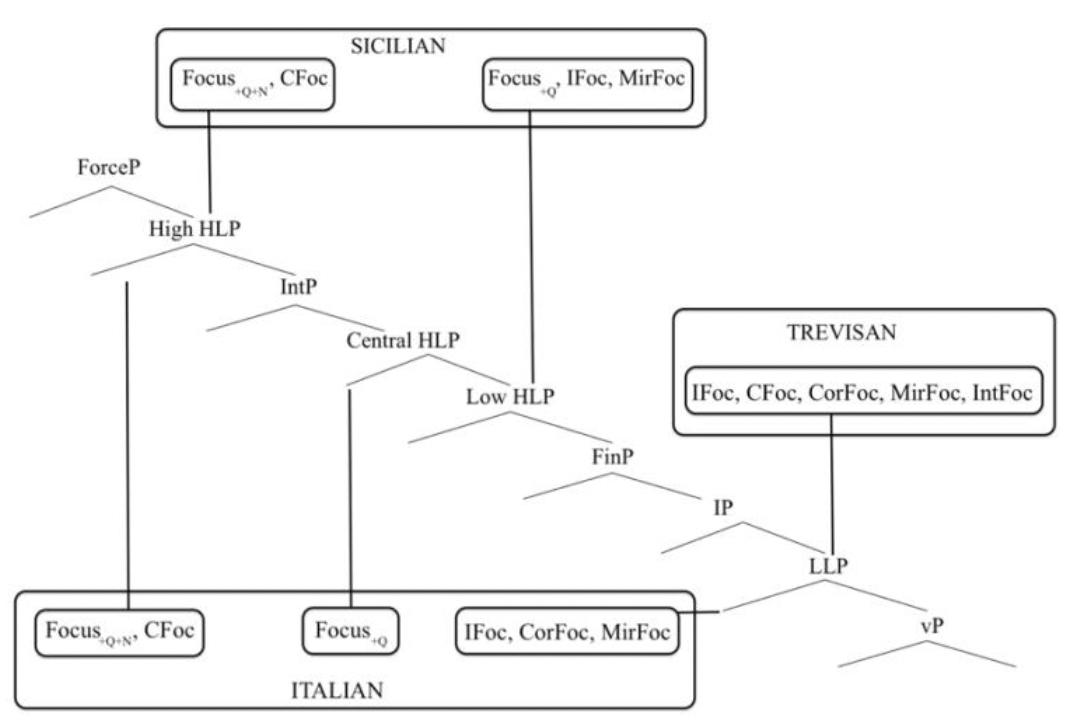
\includegraphics[width=90mm]{images/focus.png}
    \caption{Merging sites for focus projections in 3 Italo-Romance languages (Bonan (to appear)).}
    \label{fig:focus}
  \end{figure}

\subsection*{The cartography of clefts}

\citeauthor{belletti2015}’s (\citeyear{belletti2015}) cartography of clefts derives these structures utilising, depending on the nature of the structure, either \citeauthor{rizzi1997fine}’s (\citeyear{rizzi1997fine}) FocusP or \citeauthor{belletti2004}’s (\citeyear{belletti2004}) Foc. 
In both cases, the involved projections require overt movement of the focused element (IM=1), i.e. IM=1.

\begin{exe}
    \ex {[}\textsubscript{ForceP} ... {[}\textsubscript{F2b} {[}\textsubscript{FinP} {[}\textsubscript{TP} COP\textsubscript{i} {[}\textsubscript{F1b} \{focus\}\textsubscript{j} {[}\textsubscript{vP} \_\_\textsubscript{j} {[}\textsubscript{F2} \{focus\}\textsubscript{i} {[}\textsubscript{FinP} {[}\textsubscript{TP} {[}\textsubscript{F1} {[}\textsubscript{vP} ... \_\_\textsubscript{i} {]]]]]]]]]}
\end{exe}

\begin{exe}
    \ex	Subject cleft (high left-peripheral focus position in embedded clause, F2)
        \gll {[} C'est {[}\textsubscript{F1b} \textsc{jean} {[} qui me l'a dit {]]}\\
        {} ce$=$is  {}		John	{}	who to.me it$=$has told {}\\
        \vspace*{-3mm}
        \glt ‘Lit: It is \textsc{john} who told me.’
\end{exe}

\begin{exe}
    \ex	Non-subject cleft (low peripheral focus position in higher clause, F1b)
        \gll {[} C'est {[}\textsubscript{F1b} \textsc{à} \textsc{jean} {[} que je l'ai dit {]]}\\
        {} ce$=$is 		{}	to John			{}		that I it$=$have told {} \\
        \vspace*{-3mm}
        \glt ‘Lit: It is \textsc{to john} that I told (this).’
\end{exe}


\begin{table}[H]
    \centering
    \begin{tabular}{|l|l|l|l|l|l|l|}
    \hline
    & Merge & Spell Out & Search & IM & Search\textsubscript{lex} & IM\textsubscript{lex} \\
    \hline
    F2 & 1 & 0 & 1 & 0 & 0 & 0 \\
    \hline
    F1\textsubscript{b} & 1 & 0 & 1 & 0 & 0 & 0 \\
    \hline
    \end{tabular}
    \caption{\label{tab:belletti}Parametric settings for the French FocusP: VS.}
\end{table}

\noindent Based on Table 2, the discussion in the next section, and our results, we shall suggest that the projections involved in Belletti's derivation are indeed focal, but not FocusP and Foc.

\subsection*{FocusP}

FocusP has traditionally been considered responsible for the attraction of either wh-elements or contrastive foci. 
However, while the former are systematically attracted into SpecFocusP in Standard Italian, which suggests a setting as IM=1, the latter can surface either fronted or in situ (\citealt{bianchi2013}), rather suggesting an IM=1/0 setting. 

\begin{exe}
    \ex
        \begin{xlist}
            \ex \gll Cos'hai mangiato?\\
            what$=$have\textsubscript{2PS} eaten\\
            \ex \gll * Hai mangiato cosa?\\
            {} have\textsubscript{2PS} eaten what\\
            \glt \hspace{2mm} 'What did you eat?'
        \end{xlist}
\end{exe}

\begin{table}[H]
    \centering
    \begin{tabular}{|l|l|l|l|l|l|}
    \hline
    Merge & Spell Out & Search & IM & Search\textsubscript{lex} & IM\textsubscript{lex} \\
    \hline
    1 & 0 & 1 & 1 & 0 & 0 \\
    \hline
    \end{tabular}
    \caption{\label{tab:samp}Parametric settings for the Italian projection responsible for interrogative wh-movement.}
\end{table}

\begin{exe}
    \ex
        \begin{xlist}
            \ex \gll \textsc{una} \textsc{mela} ho mangiato, non un gelato!\\
            an apple have\textsubscript{1PS} eaten not an ice-cream\\
            \glt 'Lit: \textsc{an} \textsc{apple} I ate, not an ice-cream!'
            \ex \gll Ho mangiato \textsc{una} \textsc{mela}, non un gelato!\\
            have\textsubscript{1PS} eaten an apple not an ice-cream\\
            \glt 'I ate \textsc{an} \textsc{apple}, not an ice-cream!'
        \end{xlist}
\end{exe}

\begin{table}[H]
    \centering
    \begin{tabular}{|l|l|l|l|l|l|}
    \hline
    Merge & Spell Out & Search & IM & Search\textsubscript{lex} & IM\textsubscript{lex} \\
    \hline
    1 & 0 & 0/1 & 1 & 0 & 0 \\
    \hline
    \end{tabular}
    \caption{\label{tab:samp}Parametric settings for the Italian projection responsible for contrastive focus.}
\end{table}

\noindent The focus projections defined in Table 3 and 4 cannot be the same.

\noindent Clefts are present in the language but require certain context conditions to be met to be licensed (\citealt{larrive2022}). 

\noindent Languages like European French, on the other hand, have both shifted and in situ wh-elements (IM=1/0) but no prosodic foci, and productive clefts. 

\begin{exe}
    \ex
        \begin{xlist}
            \ex  \gll Quand (est-ce que) tu l'as vu?\\
            when (est-ce que) you it$=$have\textsubscript{2PS} seen\\
            \ex  \gll Tu l'as vu quand?\\
            you it$=$have\textsubscript{2PS} seen when\\
            \glt 'When did you see him?'
        \end{xlist}
\end{exe}

\begin{table}[H]
    \centering
    \begin{tabular}{|l|l|l|l|l|l|}
    \hline
    Merge & Spell Out & Search & IM & Search\textsubscript{lex} & IM\textsubscript{lex} \\
    \hline
    1 & 0 & 0/1 & 1 & 0 & 0 \\
    \hline
    \end{tabular}
    \caption{\label{tab:samp}Parametric settings for the Italian projection responsible for interrogative wh-movement.}
\end{table}

\subsection*{Foc}

The existence of Foc was originally posited to account for the existence of VS structures in Standard Italian (\citealt{belletti2004}) but many pieces of research have suggested that Italian low foci are always unmoved (\citealt{cardinaletti2001,sameklodovici15,bonan21}), thus suggesting an IM=0 setting for the language. 

\begin{exe}
    \ex Low focus in Italian
    \begin{xlist}
    \ex Question: Who's arrived?
    \ex \gll Answer A: ?? \textsc{gianni} è arrivato\\
    {} {} {} John is arrived\\
    \ex \gll Answer B: È arrivato \textsc{gianni}\\
    {} {} is arrived John\\ 
    \glt \hspace{16mm} '\textsc{john} arrived' (Lit: 'Arrived John')
    \end{xlist}
\end{exe}

\begin{exe}
    \ex VS structure in Trevisan\footnote{See Bonan(2021) for independent evidence that these orders are not a consequence of rightward movement of what follows the focus.}
        \begin{xlist}
            \ex Question: To whom did you give your snack?
            \ex \gll ?? Ghe go dato a marenda \textsc{a} \textsc{giani}\\
            {} 3dat have\textsubscript{1PS} given the snack to John\\
            \ex \gll Ghe go dato \textsc{a} \textsc{giani} a marenda\\
            3dat have\textsubscript{1PS} given to John the snack\\
            \glt 'Lit: I gave \textsc{to} \textsc{john} my snack.'
        \end{xlist}
\end{exe}

\begin{exe}
    \ex VS structure in Italian (ii)
        \begin{xlist}
            \ex Question: To whom did you give your snack?
            \ex \gll * Ho dato \textsc{a} \textsc{gianni} la merendina\\
            {} have\textsubscript{1PS} given to John the snack\\
            \ex \gll Ho dato la merendina \textsc{a} \textsc{gianni}\\
            have\textsubscript{1PS} given the snack to John\\
            \glt 'I gave the snack \textsc{to} \textsc{john}'
        \end{xlist}
\end{exe}

According to \citet{bonan22}, the different parametric settings for the low Foc in Italian vs Trevisan can be understood as in Table II:

\begin{table}[ht]
    \centering
    \begin{tabular}{|l|l|l|l|l|l|l|}
    \hline
     & Merge & Spell Out & Search & IM & Search\textsubscript{lex} & IM\textsubscript{lex} \\
    \hline
    Italian & 1 & 0 & 1 & 0 & 0 & 0 \\
    \hline
    Trevisan & 1 & 0 & 1 & 1 & 0 & 0\\
    \hline
    \end{tabular}
    \caption{\label{tab:samp2}Language variability in activating FocP.}
    \end{table}

\noindent In French, the low focus position is not exploited in any known structure.

\section*{4. Working hypotheses}
The working hypotheses behind the present study are as follows:

\begin{itemize}
\item The parametrisation of functional projections evolves in the direction of no movement (IM=0 in \citeauthor{rizzi2017}’s \citeyear{rizzi2017} terms, see works on the diachrony of Chinese interrogatives \citealt{aldridge2010clause} or Japanese, \citealt{aldridge2009old}, but also \citealt{roberts2003syntactic}, \citealt{dadan2019}, a.o.).

\begin{table}[ht]
    \centering
    \begin{tabular}{|l|l|l|l|l|l|l|}
    \hline
     & Merge & Spell Out & Search & IM & Search\textsubscript{lex} & IM\textsubscript{lex} \\
    \hline
    Archaic Chinese ($=$Trevisan) & 1 & 0 & 1 & 0 & 0 & 0\\
    \hline
    Heian Chinese & 1 & 0 & 1 & 0/1 & 0 & 0 \\
    \hline
    Contemporary Chinese ($=$Italian) & 1 & 0 & 1 & 1 & 0 & 0 \\
    \hline
    \end{tabular}
    \caption{\label{tab:samp2}Parametrisations of FocP in the evolution of Chinese.}
    \end{table}

\item Diachronically, one functional projection can display different settings for the same parameter at different stages (cf. IM in Table 7);

\item When what is commonly considered as one single projection displays different parametrisations across structures (e.g., IM=1 in clefts vs IM=0 in interrogatives), the existence of two separate projections ought to be posited instead (e.g., clefts).
\end{itemize}

\section*{5. Methodology}

Our hypotheses are being tested utilising corpus linguistics techniques.\footnote{The project repo is publicly available https://github.com/CaterinaBi/parameters-corpus-work.}
 
As a preliminary assessment of the theory, we have limited the scope of the present investigation to the study of three standard Romance languages: Italian, French and European Portuguese. 

\noindent The corpora used for this part of the study are: 

\begin{itemize}
\item[\ding{227}] \vspace*{-2mm} ESLO 1 and ESLO2 (spoken French, 1970-2014) (data from Baunaz \& Bonan (in prep.));
\item[\ding{227}] \vspace*{-2mm} Bonan's corpus of 485 theatre scripts (late 1500-early 1900).\footnote{The data can be retrieved at https://github.com/CaterinaBi/parameters-corpus-work/tree/main/raw_data_theatre/data.}
\end{itemize}

\noindent The data were pre-classified automatically (position of the wh-element, interrogative strategy, well-formedness, position), then checked manually.
\noindent Here, we present our preliminary data on French interrogatives. This only includes:
\begin{itemize}
    \item[\ding{227}] \vspace*{-2mm} well-formed clauses (no fragments, no questions containing only a wh-element);
    \item[\ding{227}] \vspace*{-2mm} wh-questions;
    \item[\ding{227}] \vspace*{-2mm} matrix questions.
\end{itemize}

\section*{7. Preliminary results for French}

\subsection*{From predominant ex situ to predominant in situ}

\begin{table}[H]
    \centering
    \small
    \begin{adjustbox}{width=\textwidth}
        \begin{tabular}{l|ll|ll|ll|ll|ll|ll}
        % \hline
        {} & \multicolumn{2}{c}{comment}  & \multicolumn{2}{c}{où} & \multicolumn{2}{c}{quand}& \multicolumn{2}{c}{quiS} & \multicolumn{2}{c}{quiO}& \multicolumn{2}{c}{quoiO}\\
        \hline
        {} & EX & IN & EX & IN & EX & IN & EX & IN & EX & IN & EX & IN\\
        %\hline
        1870$-$1900 & 60 & 0 & 102 & 0 & 14 & 0 & 94 & 0 & 15 & 0 & 36 & 0\\
        %\hline
        1900$-$1930 & 40 & 0 & 39 & 0 & 4 & 0 & 33 & 0 & 9 & 0 & 17 & 0\\
        %\hline
        1970 (eslo 1) & 848 & 37 & 233 & 72 & 156 & 38 & 416 & 4 & 42 & 13 & 333 & 198\\
        %\hline
        2014 (eslo 2) & 333 & 156 & 84 & 260 & 32 & 30 & 86 & 6 & 8 & 21 & 24 & 476 \\
        \hline
        \end{tabular}
    \end{adjustbox}
\caption{\label{tab:samp3}Total occurrences of non lexically-restricted wh-elements.}
\end{table}

\begin{figure}[h!]
    \centering
    \begin{subfigure}[b]{0.49\linewidth}
      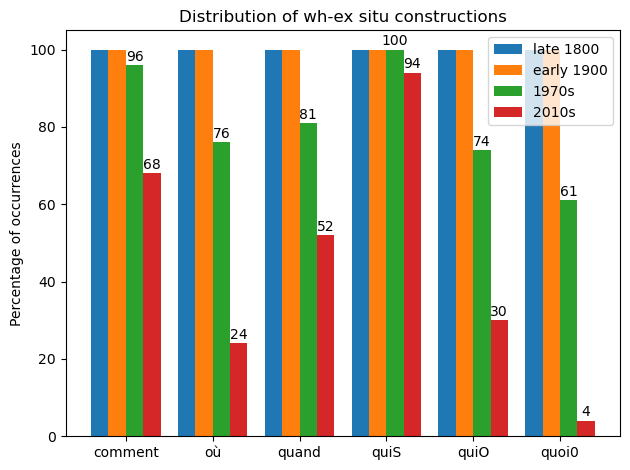
\includegraphics[width=\linewidth]{images/exsitu.png}
      %\caption{Coffee.}
    \end{subfigure}
    \begin{subfigure}[b]{0.49\linewidth}
      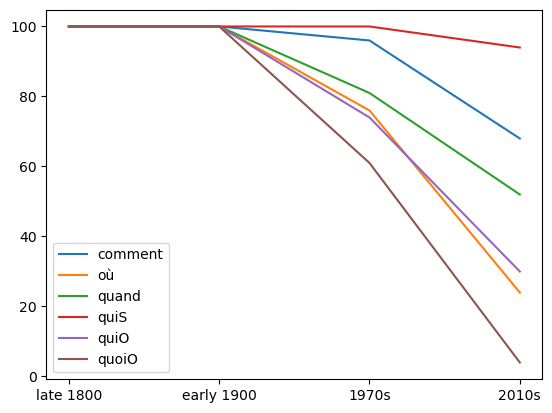
\includegraphics[width=\linewidth]{images/exsitu2.png}
      % \caption{More coffee.}
    \end{subfigure}
    \caption{Evolution of the distribution of wh-ex situ structures.}
    \label{fig:ex situ}
  \end{figure}

  \begin{figure}[h!]
      \centering
      \begin{subfigure}[b]{0.49\linewidth}
        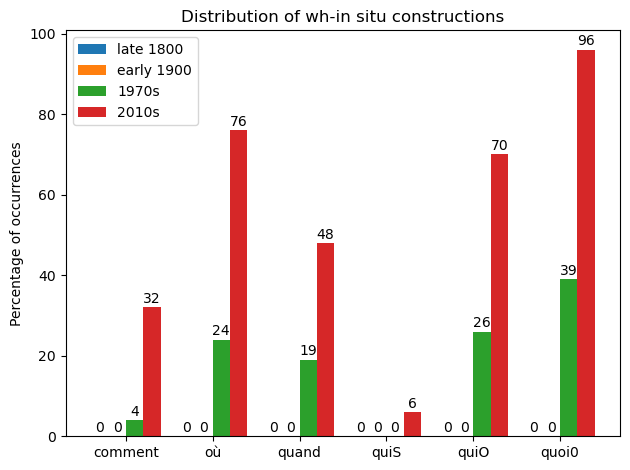
\includegraphics[width=\linewidth]{images/insitu.png}
        %\caption{Coffee.}
      \end{subfigure}
      \begin{subfigure}[b]{0.49\linewidth}
        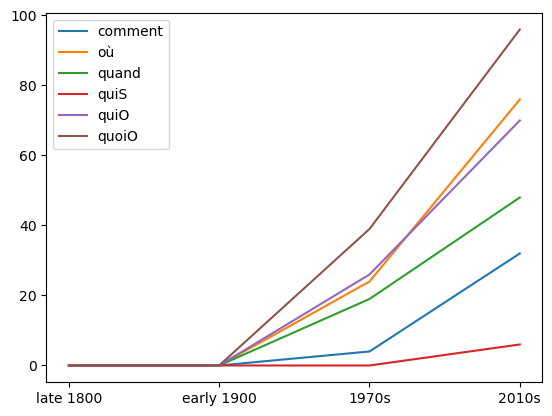
\includegraphics[width=\linewidth]{images/insitu2.png}
        % \caption{More coffee.}
      \end{subfigure}
      \caption{Evolution of the distribution of wh-in situ structures.}
      \label{fig:in situ}
    \end{figure}

\noindent What this means in our framework (the 'n/a' parameters will be discussed in the following two sections):

    \begin{table}[H]
        \centering
        \begin{tabular}{|l|l|l|l|l|l|l|}
        \hline
         & Merge & Spell Out & Search & IM & Search\textsubscript{lex} & IM\textsubscript{lex} \\
        \hline
        late 1800 & 1 & n/a & 1 & 0 & n/a & n/a \\
        \hline
        early 1900 & 1 & n/a & 1 & 0 & n/a & n/a \\
        \hline
        1970s & 1 & n/a & 1 & 0/1 & n/a & n/a \\
        \hline
        2010s & 1 & n/a & 1 & 0/1 & n/a & n/a \\
        \hline
        \end{tabular}
        \caption{\label{tab:samp}Parametric settings for the French FocusP: evolution over time.}
    \end{table}

\noindent Our understanding of French interrogative wh-movement:
    \begin{enumerate}
        \item French was a wh-fronting language (IM=0 for FocusP) up until at least the beginning of the 20\textsuperscript{th} century;
        \item \vspace*{-2mm} French has been characterized by movement optionality (IM=0/1) since at least the beginning of the 1970s;
        \item \vspace*{-2mm} French will evolve to either:
        \begin{itemize}
            \item \vspace*{-2mm} lose fronting altogether (IM=0);
            \item \vspace*{-2mm} develop a specialised meaning for each strategy (cf. Palasis \& Faure 2021).
        \end{itemize}    
    \end{enumerate}

\subsection*{From verb movement and head activation to predominant non-movement/activation}

The case of VS structure vs SV structures.

\begin{table}[H]
    \centering
    \small
    \begin{adjustbox}{width=\textwidth}
        \begin{tabular}{l|ll|ll|ll|ll|ll}
        % \hline
        {} & \multicolumn{2}{c}{comment}  & \multicolumn{2}{c}{où} & \multicolumn{2}{c}{quand} & \multicolumn{2}{c}{quiO}& \multicolumn{2}{c}{quoiO}\\
        \hline
        {} & VS & SV & VS & SV & VS & SV & VS & SV & VS & SV\\
        %\hline
        1870$-$1900 & 58 & 2 & 81 & 4 & 11 & 3 & 13 & 1 & 29 & 6\\
        %\hline
        1900$-$1930 & 35 & 5 & 35 & 3 & 3 & 1 & 8 & 1 & 17 & 0\\
        %\hline
        1970 (eslo 1) & 144 & 435 & 41 & 105 & 62 & 55 & 14 & 23 & 90 & 319 \\
        %\hline
        2014 (eslo 2) & 28 & 457 & 12 & 295 & 4 & 45 & 1 & 26 & 2 & 537 \\
        \hline
        \end{tabular}
    \end{adjustbox}
\caption{\label{tab:samp6}Total occurrences of VS and SV (includes ex situ and in situ constructions).}
\end{table}

\begin{figure}[h!]
    \centering
    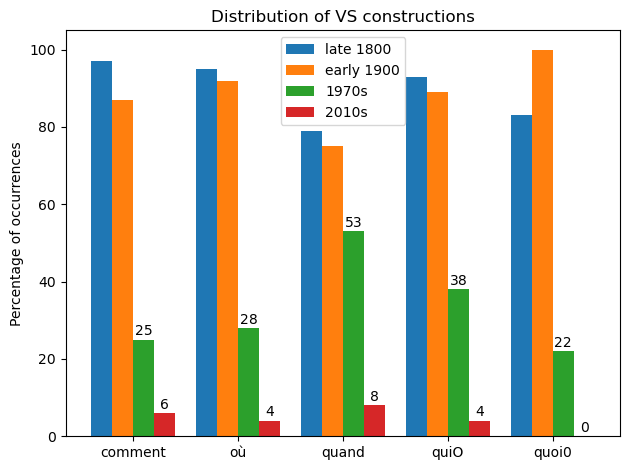
\includegraphics[width=90mm]{images/VS.png}
    \caption{Distribution of VS structures wrt all SV structures.}
    \label{fig:boat1}
  \end{figure}

  \begin{figure}[H]
    \centering
    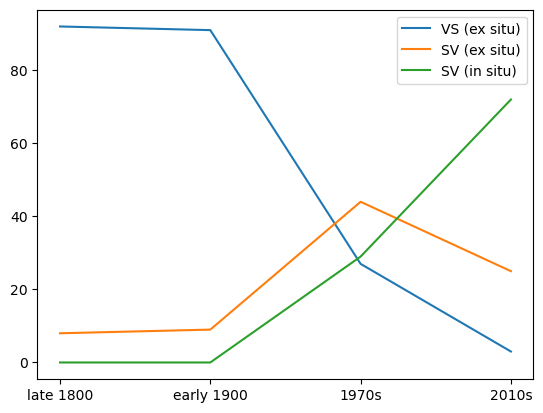
\includegraphics[width=90mm]{images/exsituinsitu.png}
    \caption{Distribution of VS structures wrt ex situ SV and in situ SV structures.}
    \label{fig:boat2}
  \end{figure}

  \noindent What this means in our framework:

  \noindent Two possible parametrisations coexist.
  
  \noindent Up until at least the 1930s, French required spelling out the head of Focus (SpellOut=1, see Roberts 2017 for an understanding of French enclitics as an inflectional class) and merging the finite verb (IM\textsubscript{lex}) almost systematically.

    \begin{table}[H]
        \centering
        \begin{tabular}{|l|l|l|l|l|l|}
        \hline
        Merge & Spell Out & Search & IM & Search\textsubscript{lex} & IM\textsubscript{lex} \\
        \hline
        1 & 1 & 1 & 0 & 1 & 1 \\
        \hline
        \end{tabular}
        \caption{\label{tab:samp}Parametric settings for the French FocusP: VS.}
    \end{table}

\noindent The option of not spelling out Focus^0 (SpellOut=0) existed, but was still rare. This systematically correlates to no movement of the finite verb (IM\textsubscript{lex}=0).

\begin{table}[H]
    \centering
    \begin{tabular}{|l|l|l|l|l|l|}
    \hline
    Merge & Spell Out & Search & IM & Search\textsubscript{lex} & IM\textsubscript{lex} \\
    \hline
    1 & 0 & 1 & 0 & 0 & 0 \\
    \hline
    \end{tabular}
    \caption{\label{tab:samp}Parametric settings for the French FocusP: SV.}
\end{table}

\noindent The parametrisation in Table X became dominant before the 1970s.

\noindent Forecasted possible evolution: total loss of VS.

\subsection*{From verb movement to predominant non-movement}

'Est-ce que/i' structures can be understood as a case of IM\textsubscript{lex}=1. While head Spell Out cannot exist in the absence of verb movement (VS, see above), verb movement does not require spelling out of the head.

\begin{table}[H]
    \centering
    \large
        \begin{tabular}{l|l|l|l|l|l|l}
        \hline
        {} & comment & où & quand & quiS & quiO & quoiO \\
        %\hline
        1870$-$1900 & 0 & 0 & 0 & 7 & 7 & 0 \\
        %\hline
        1900$-$1930 & 0 & 1 & 0 & 8 & 0 & 0 \\
        %\hline
        1970 (eslo 1) & 286 & 157 & 77 & 163 & 13 & 136 \\
        %\hline
        2014 (eslo 2) & 44 & 35 & 13 & 17 & 0 & 0 \\
        \hline
        \end{tabular}
\caption{\label{tab:samp8}Total occurrences of VS and SV (includes ex situ and in situ constructions).}
\end{table}

\begin{figure}[H]
    \centering
    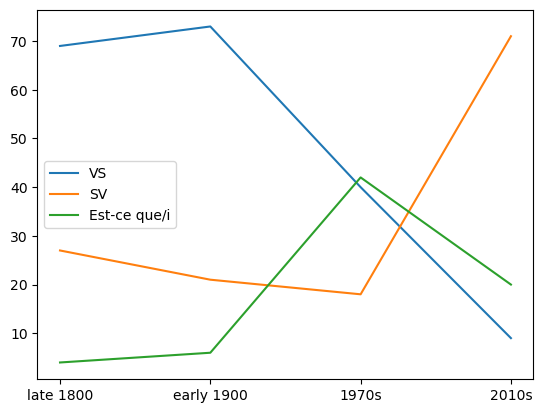
\includegraphics[width=90mm]{images/estceque.png} % possibility to print est-ce que alone
    \caption{Distribution of 'est-ce que' in constructions with the wh-elements in Table 6.}
    \label{fig:boat4}
  \end{figure}


  \noindent Est-ce que data in Table 6 seem to suggest that est-ce que was not productive in late 1800, contrary to fact.
  \noindent This is due to the fact that this presentation does not include the data for 'qu(e)'.

  Data already collected for 'qu(e)':
  \begin{enumerate}
    \item late 1800: 'qu(e)' constitutes 55\% of all occurrences:
        \begin{itemize}
            \item[\ding{227}] \vspace*{-2mm} Que VS: 43\%;
            \item[\ding{227}] \vspace*{-2mm} Qu' VS: 26\%;
            \item[\ding{227}] \vspace*{-2mm} Qu'est-ce que: 31\%.
        \end{itemize}
    \item early 1900: 'qu(e)' constitutes 64\% of all occurrences:
        \begin{itemize}
            \item[\ding{227}] \vspace*{-2mm} Que VS: 19\%;
            \item[\ding{227}] \vspace*{-2mm} Qu' VS: 13\%;
            \item[\ding{227}] \vspace*{-2mm} Qu'est-ce que: 68\%.
        \end{itemize}
\end{enumerate}

  \begin{figure}[H]
    \centering
    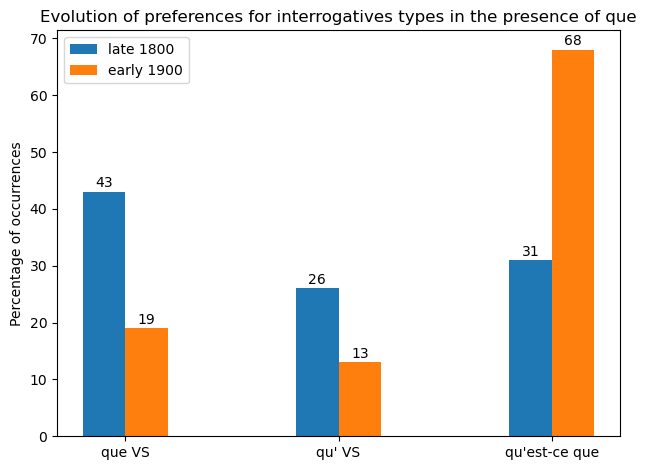
\includegraphics[width=90mm]{images/que.png} % possibility to print est-ce que alone
    \caption{Evolution of preferences for interrogatives types in the presence of que.}
    \label{fig:boat5}
  \end{figure}

\noindent What this means in our framework:

\noindent There is a third configuration to be added to those in §X. This, as the configuration in Table X (VS), is becoming less common today compared to SV:

\begin{table}[H]
    \centering
    \begin{tabular}{|l|l|l|l|l|l|}
    \hline
    Merge & Spell Out & Search & IM & Search\textsubscript{lex} & IM\textsubscript{lex} \\
    \hline
    1 & 0 & 1 & 0 & 1 & 1 \\
    \hline
    \end{tabular}
    \caption{\label{tab:samp}Parametric settings for the French FocusP: est-ce que.}
\end{table}

\noindent Possible evolutions:

\begin{enumerate}
    \item \vspace*{-2mm} total loss of est-ce que structures;
    \item \vspace*{-2mm} specialisation of est-ce que structures and peaceful coexistence with SV.
\end{enumerate}

\subsection*{Further steps}

The data presented today is only a fraction of the work that we have been doing and plan to do. Certain implementations will include:
\begin{enumerate}
    \item cleaning and analysis of data for 'qu(e)' in eslo1/2 \& adjust calculations;
    \item \vspace*{-2mm} observation of the evolution from SVS ('Quand Jean a-t-il appelé?') to VS(S) structures ('Quand a-t-il appelé (Jean)?') from 1600 to 2010s; 
    \item \vspace*{-2mm} observation of the evolution from Wh>Cop interrogative clefts ('Quand c'est qu'il a appelé?') to Cop>Wh ('C'est quand qu'il a appelé?'). For now, we have observed the following:
    \begin{itemize}
        \item[\ding{227}] \vspace*{-2mm} biclausal interrogative clefts are scarce (DATA);
        \item[\ding{227}] \vspace*{-2mm} in late 1800, no clefts were found;
        \item[\ding{227}] \vspace*{-2mm} in early 1900, only complex clefts of the 'qu'est-ce que c'est que [...]' type were observed.
        \item[\ding{227}] \vspace*{-2mm} in the 1970s, Cop>Wh clefts were already dominant (DATA), although also WH>Cop clefts were present.
        \item[\ding{227}] \vspace*{-2mm} in the 2010s, Cop>Wh clefts were not attested.
    \end{itemize}
    \item \vspace*{-2mm} repetition of the experience for Italian and Portuguese. 
\end{enumerate}

\section*{Conclusions}

\begin{itemize}
\item[\ding{227}] French wh-interrogatives have evolved in the direction of no IM, no SO and no IM\textsubscript{lex}, as per our working hypotheses;
\item[\ding{227}] \vspace*{-2mm} the parametrization of the projection responsible for interrogative wh-movement in French is evolving towards IM=0 and is at present at the optionality stage seen for Heian Chinese (IM=0/1).
\item[\ding{227}] \vspace*{-2mm} because of the previous point, and the fact that the low FocP has IM=0 in French, it is undesirable to classify the projections involved in the derivation of clefts as FocusP (IM=0/1 for foci) and FocP (IM=0);
\item[\ding{227}] \vspace*{-2mm} Rizzi's (2017) elegant understanding of parameters allows for fine descriptions of how functional projections work, and evolve over time;
\item[\ding{227}] \vspace*{-2mm} simple observations like the ones in this study can allow the splitting of projections previously believed to be a single projection.
\end{itemize}

\bibliography{sample}

\section*{Acknowledgements}

\end{document}
